\clearpage
\section{Edge-based variables}
\label{sec:edge-based}

In all figures in this subsection, the reader should focus on red parts.
Black ones refer to cell-based variables and are kept for reference only.

%%%%%%%%%%%%%%%%%%%%%%%%%
%                       %
%  Sequential Periodic  %
%                       %
%%%%%%%%%%%%%%%%%%%%%%%%%
\subsection{Sequential Periodic}

\subsubsection{Numeration}

%-------------%
%             %
% Edge 1.1.1. %
%             %
%-------------%
\begin{figure}[h]
  \centering
  \setlength{\unitlength}{1mm}
  \begin{picture}(105,70)(0,0)
    \thickbox{105}{70}
    \put( 1,0){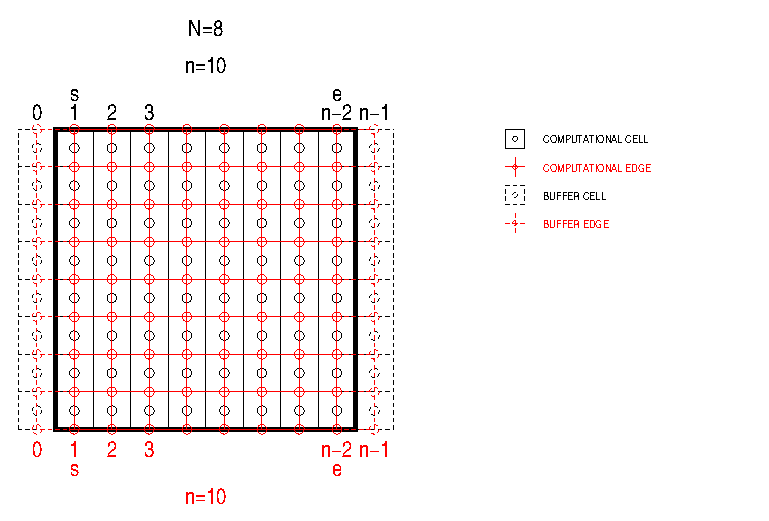
\includegraphics[scale=0.85]{Figures/Edge/1periodic_1sequential_1numeration.eps}}
  \end{picture}
  \caption{Numeration of sequential edge-based variable with periodic boundary 
           condition.}
  \label{edge:111}
\end{figure}

Description of Fig.~\ref{edge:111}:
\begin{enumerate}
  \item Numeration of the edge-based variable for horizontal direction is 
        the same as for cell-based variables described in Sec.~\ref{sec:cell-based}.
  \item As a consequence, everything said for Fig.~\ref{cell:111} holds here too.
\end{enumerate}

\clearpage
\subsubsection{Communication}

%-------------%
%             %
% Edge 1.1.2. %
%             %
%-------------%
\begin{figure}[h]
  \centering
  \setlength{\unitlength}{1mm}
  \begin{picture}(105,65)(0,0)
    \thickbox{105}{65}
    \put( 1,0){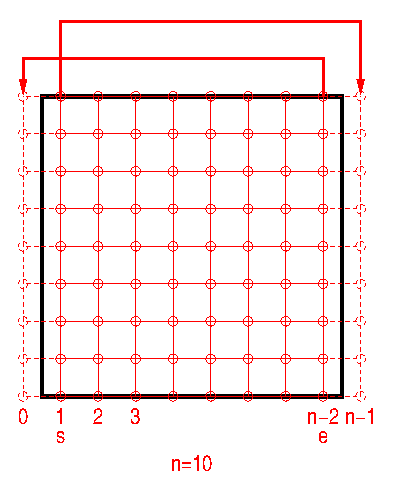
\includegraphics[scale=0.85]{Figures/Edge/1periodic_1sequential_2patterns.eps}}
  \end{picture}
  \caption{Communication patterns for sequential edge-based variable with 
           periodic boundary condition.}
  \label{edge:112}
\end{figure}

Description of Fig.~\ref{edge:112}: Same as for Fig.~\ref{cell:112}.

%%%%%%%%%%%%%%%%%%%%%%%
%                     %
%  Parallel Periodic  %
%                     %
%%%%%%%%%%%%%%%%%%%%%%%
\clearpage
\subsection{Parallel Periodic}

\subsubsection{Numeration}

%-------------%
%             %
% Edge 1.2.1. %
%             %
%-------------%
\begin{figure}[ht]
  \centering
  \setlength{\unitlength}{1mm}
  \begin{picture}(105,145)(0,0)
    \thickbox{105}{145}
    \put( 1,0){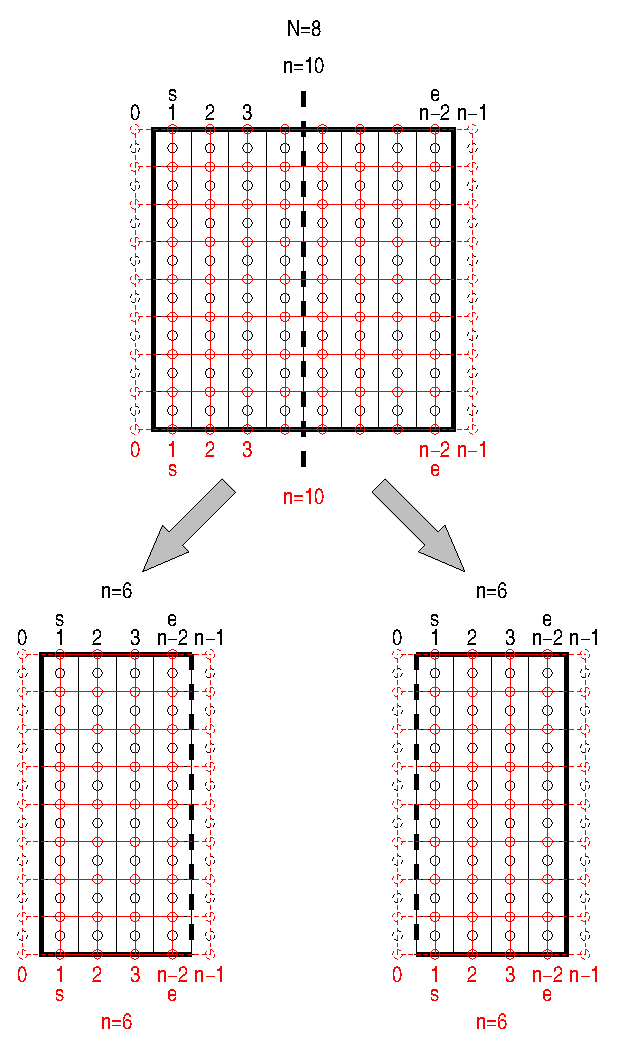
\includegraphics[scale=0.85]{Figures/Edge/1periodic_2parallel_1numeration.eps}}
  \end{picture}
  \caption{Numeration of edge-based variable with periodic boundary 
           condition for parallel computation.}
  \label{edge:121}
\end{figure}

Description of Fig.~\ref{edge:121}: Same as for Fig.~\ref{cell:121}.

\clearpage
\subsubsection{Communication}

%-------------%
%             %
% Edge 1.2.2. %
%             %
%-------------%
\begin{figure}[ht]
  \centering
  \setlength{\unitlength}{1mm}
  \begin{picture}(105,75)(0,0)
    \thickbox{105}{75}
    \put( 1,0){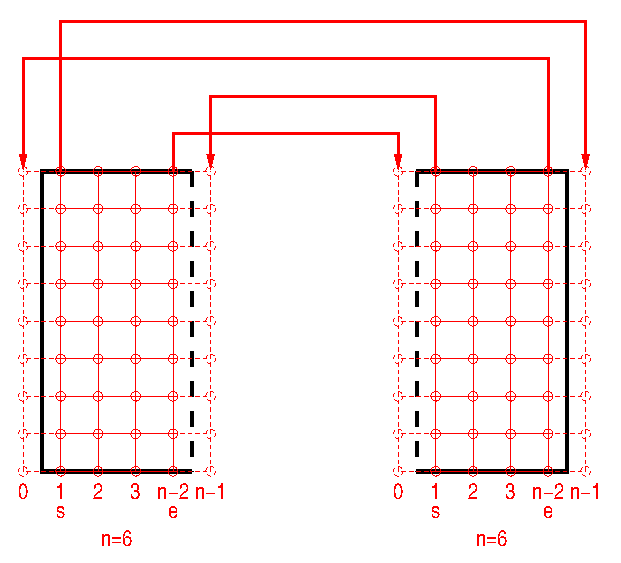
\includegraphics[scale=0.85]{Figures/Edge/1periodic_2parallel_2patterns.eps}}
  \end{picture}
  \caption{Communication patterns for parallel edge-based variable with 
           periodic boundary condition.}
  \label{edge:122}
\end{figure}

Description of Fig.~\ref{edge:122}: Same as for Fig.~\ref{cell:122}.

%%%%%%%%%%%%%%%%%%%%%%%%%%%%%
%                           %
%  Sequential Non-periodic  %
%                           %
%%%%%%%%%%%%%%%%%%%%%%%%%%%%%
\subsection{Sequential Non-periodic}

\subsubsection{Numeration}

%-------------%
%             %
% Edge 2.1.1. %
%             %
%-------------%
\begin{figure}[ht]
  \centering
  \setlength{\unitlength}{1mm}
  \begin{picture}(105,70)(0,0)
    \thickbox{105}{70}
    \put( 1,0){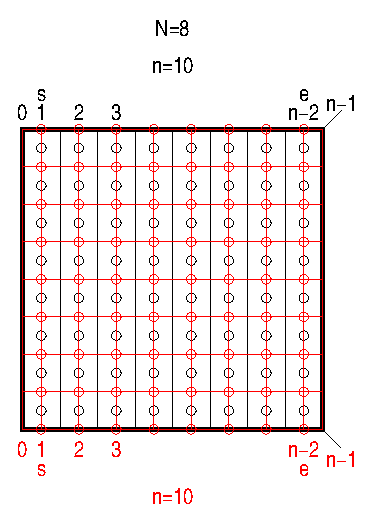
\includegraphics[scale=0.85]{Figures/Edge/2non-periodic_1sequential_1numeration.eps}}
  \end{picture}
  \caption{Numeration of sequential edge-based variable with non-periodic boundary
           condition.}
  \label{edge:211}
\end{figure}

Description of Fig.~\ref{edge:211}: Same as for Fig.~\ref{cell:211}.

%%%%%%%%%%%%%%%%%%%%%%%%%%%
%                         %
%  Parallel Non-periodic  %
%                         %
%%%%%%%%%%%%%%%%%%%%%%%%%%%
\subsection{Parallel Non-periodic}

\subsubsection{Numeration}

%-------------%
%             %
% Edge 2.2.1. %
%             %
%-------------%
\begin{figure}[ht]
  \centering
  \setlength{\unitlength}{1mm}
  \begin{picture}(105,145)(0,0)
    \thickbox{105}{145}
    \put( 1,0){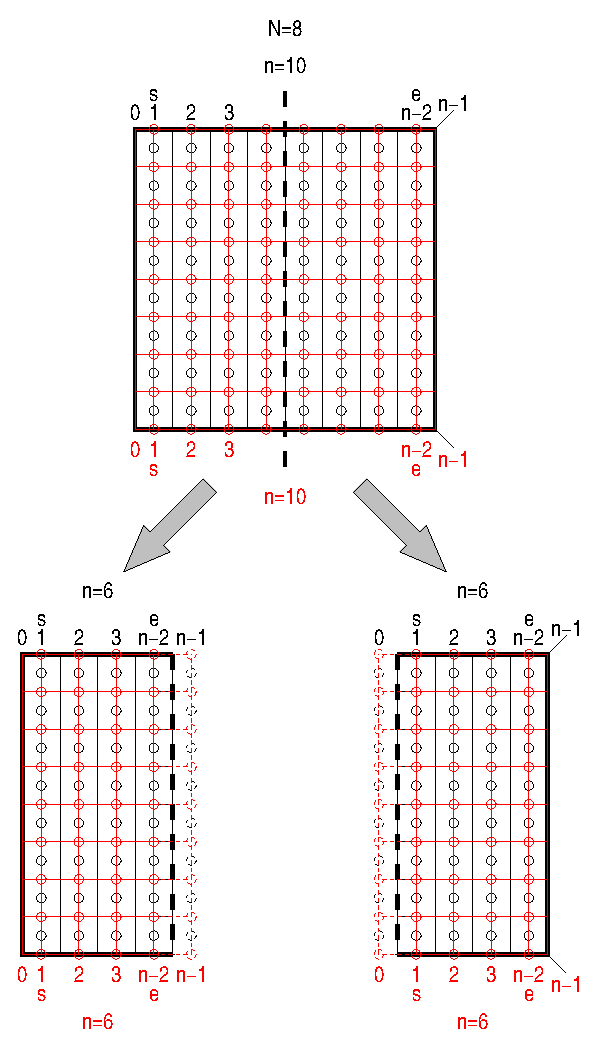
\includegraphics[scale=0.85]{Figures/Edge/2non-periodic_2parallel_1numeration.eps}}
  \end{picture}
  \caption{Numeration of sequential edge-based variable with non-periodic boundary
           condition.}
  \label{edge:221}
\end{figure}

Description of Fig.~\ref{edge:221}: Same as for Fig.~\ref{cell:221}.

\clearpage
\subsubsection{Communication}

%-------------%
%             %
% Edge 2.2.2. %
%             %
%-------------%
\begin{figure}[ht]
  \centering
  \setlength{\unitlength}{1mm}
  \begin{picture}(105,65)(0,0)
    \thickbox{105}{65}
    \put( 1,0){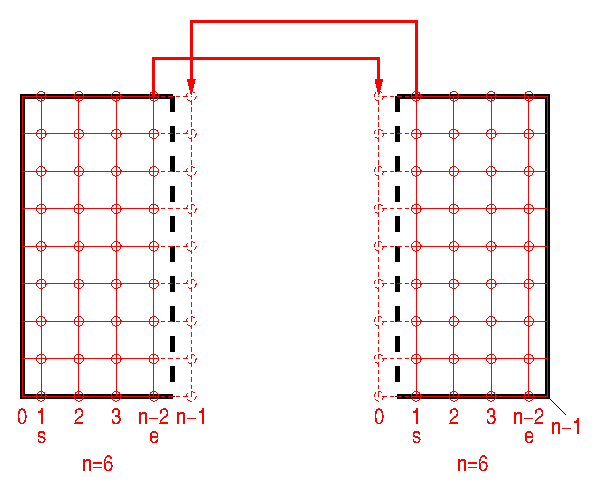
\includegraphics[scale=0.85]{Figures/Edge/2non-periodic_2parallel_2patterns.eps}}
  \end{picture}
  \caption{Communication patterns for parallel edge-based variable with 
           periodic boundary condition.}
  \label{edge:222}
\end{figure}

Description of Fig.~\ref{edge:222}: Same as for Fig.~\ref{cell:222}.

%------------------------------------------------------------------------notes-%
\vspace*{5mm} \fbox{ \begin{minipage}[c] {0.97\textwidth} %--------------notes-%
    {\sf Note on other coordinate directions} \\ %-----------------------notes-%

Edge-based variables have the same numeration and communication patterns as
cell-based ones, but the other two directions must be treated like node-based
variables explained in Sec.~\ref{sec:node-based}.

  \end{minipage} } %-----------------------------------------------------notes-%
%------------------------------------------------------------------------notes-%
